\documentclass[12pt, a4paper]{article} %determina o tamanho da fonte, o tipo de papel e o tipo de documento.

\setlength{\parindent}{1.0 cm} %tamanho do espaço para começar o parágrafo.
\setlength{\parskip}{0.5cm} %tamanho do espaço entre os parágrafos.

%Aqui ficam os pacotes utilizados para formatação do documento de modo geral:

\usepackage[utf8]{inputenc} 
\usepackage{indentfirst} %Coloca espaços nos inícios de parágrafos automaticamente. 
\usepackage[brazilian]{babel} %
\usepackage{amsmath}
\usepackage[hmargin=3cm, vmargin=2.5cm, bmargin=2.5cm]{geometry}
\usepackage{multicol}
\usepackage{graphicx} %para poder inserir imagens
\usepackage{subfig}
\usepackage{booktabs} 
\usepackage{hyperref} %para poder adicionar links e hiperlinks
\usepackage{float} %para poder posicionar as imagens
\usepackage{appendix}
\usepackage{hyperref}

\usepackage{listings} %para poder incluir códigos
\usepackage{xcolor}
\definecolor{codegreen}{rgb}{0,0.6,0}
\definecolor{codegray}{rgb}{0.5,0.5,0.5}
\definecolor{codepurple}{rgb}{0.58,0,0.82}
\definecolor{backcolour}{rgb}{0.95,0.95,0.92}
\lstdefinestyle{mystyle}{
    backgroundcolor=\color{backcolour},   
    commentstyle=\color{codegreen},
    keywordstyle=\color{magenta},
    numberstyle=\tiny\color{codegray},
    stringstyle=\color{codepurple},
    basicstyle=\ttfamily\footnotesize,
    breakatwhitespace=false,         
    breaklines=true,                 
    captionpos=b,                    
    keepspaces=true,                 
    numbers=left,                    
    numbersep=5pt,                  
    showspaces=false,                
    showstringspaces=false,
    showtabs=false,                  
    tabsize=2,
    morecomment={l}[!],
    language=[77]Fortran,
}
\lstset{style=mystyle}

\begin{document} %começa alguma coisa,neste caso, o documento, sempre importante lembrar de colocar o \end{} para não dar erro 
	
	\begin{titlepage}
		\begin{center}
\Huge{Universidade de São Paulo}\\
\large{C4AI}\\
\vspace{20pt}
\vspace{200pt}
\textbf{Sub Relat\'orios}\\
\vspace{8cm}
		\end{center}

\begin{flushleft}
\begin{tabbing}
Pedro Calligaris Delbem\\
\end{tabbing}
\vspace{0.5cm}
Orientador: Fillipo Ghiglieno\\		
		\end{flushleft}
	
		\begin{center}
			\vspace{\fill}
	Agosto de 2024
		\end{center}
	\end{titlepage}

%####################################################################### SUMÁRIO
	\tableofcontents 
	\thispagestyle{empty}
	\newpage
%#########################################################################

\section{Parte 1: Somador Completo}

    \subsection{Introdução}
    
        Para estudar o somador completo qu\^antico (quantun full adder), \'e necess\'ario - primeiro - compreender, e desenvolver, o somador completo cl\'assico.
        
        Deste modo, implementou-se o somador completo cl\'assico que consiste em um circuito que recebe dois de dois bits e um "carry in" resultando em um bit de sa\'ida e um "carry out" de modo a representar a soma de dois bits com um poss\'ivel bit extra vindo de uma soma anterior.
    
    \subsection{Materiais e Métodos}
    
        No processo utilizou-se o Intel® Quartus® Prime Lite Edition Design Software Version 21.1.1 para fazer o design de hardware além de um FPGA DE0-CV Cyclone V 5CEBA4F23C7N onde programou-se o mesmo.
    
        Primeiramente buscou-se implementar apenas uma porta "and" para compreender a utiliza\c{c}\~ao do software Quartus. Em seguida, desenvolveu-se o somador completo que funcionou perfeitamente ao ser testado na FPGA.
        
        Posteriormente buscou-se medir os tempos de rea\c{c}\~ao do hardware - ao mudar os valores de entrada - utilizando o simulador de FPGA "ModelSim", junto ao programa Quartus, mas por problemas do Software (dos quais n\~ao encontrou-se solu\c{c}\~ao) n\~ao foi realizada a simula\c{c}\~ao.
    
    \subsection{Resultados e Discussão}
    
        Na imagem 1, v\^e-se o hardware implementado para o somador completo cl\'assico
    
        \begin{figure}[H]
        \centering
        
        \includegraphics[width=1.00\textwidth]{imagens/full_adder.png}
        imagem 1: implementa\c{c}\~ao do circuito de um somador completo mo programa Quartus
        
        \end{figure}
    
    \subsection{Conclusão}
    
        O procedimento como um todo foi essencial para o desenvolver uma comprensão completa das propriedade do somador completo cl\'assico. Tais entendimentos ser\~ao fundamentais no entendimento, desenvolvimento de um somador completo qu\^antico, al\'em de possibilitar compara\c{c}\~oes entre as vantagens e desvantagens de cada um.

\section{Parte 2: Somador Completo Qu\^antico}

    \subsection{Introdução}
    
        Para desenvolver uma rede neural celular qu\^antica, faz necess\'ario entender somador completo qu\^antico. Ao contrário do caso do somador completo cl\'assico - todas as portas l\'ogicas na computa\c{c}\~ao qu\^antica devem ser revers\'iveis.
    
        Deste modo, cada opera\c{c}\~ao deve contar com um qubit auxiliar de controle que garante a reversibilidade. Buscou-se entender este processo e implementar o somador completo qu\^antico.
    
    \subsection{Materiais e Métodos}
    
        Utilizando o Circuit Composer no site da IBM, que permite utilizar as portas l\'ogicas qu\^anticas em um sistema de "arrastar" implementou-se o somador completo qu\^antico.
    
        As principais portas l\'ogicas utilizadas s\~ao Controled-NOT que dado dois qubit's retorna o inverso do qubit que n\~ao \'e o de controle e a Controled-Controled-NOT (Toffoli's Gate) que dado tr\^es qubit's retorna a adi\c{c}\~ao entre os qubit's que n\~ao s\~ao os de controle.

        Por fim, faz-se importante simular os resultados antes de process\'a-los no hardware real. Uma vez que - para circuitos mais complexos a sa\'ida correta n\~ao ser\'a t\~ao \'obvia. Ent\~ao utilizando a biblioteca "Qiskit" para Python, da IBM - foi poss\'ivel montar o mesmo circuito e simul\'a-lo atrav\'es do c\'odigo.
    
    \subsection{Resultados e Discussão}
    
        Na imagem 1, v\^e-se o hardware implementado para o somador completo 
        qu\^antico
    
        \begin{figure}[H]
        
        \centering
        
        \includegraphics[width=0.60\textwidth]{imagens/my_quantun_full_adder.png}
        
        imagem 2: implementa\c{c}\~ao do circuito de um somador completo mo IBM Circuit Composer
        
        \end{figure}
    
        Note que o qubit \'e sempre inicializado em 0, assim para utilizar o valor 1, devemos invert\^e-lo. Al\'em disso \'e not\'orio que a opera\c{c}\~ao "medida" (\'icone cinza) apensar de n\~ao-revers\'ivel \'e necess\'aria para trazermos o resultado qu\^antico para o "mundo cl\'assico".
    
        Ademais, \'e importante perceber que o uso da porta "RX(pi)" \'e necess\'ario para manter e reversibilidade do "carry out" que poder\'a ser utilizado em outra soma de quibit's.
    
        Ao rodar o circuito em um dos computadores que\^anticos da IBM, \'e sempre importante observar qual tem a menor fila de espera e foi reiniciado a menos tempo - para que se garanta um resultado com menor ru\'ido.
        
        \begin{figure}[H]
        
        \centering
        
        \includegraphics[width=1.00\textwidth]{imagens/select_quantum_computer.png}
        
        imagem 3: janela de escolha de hardware no IBM Circuit Composer
        
        \end{figure}

        Para exemplificar isso, foram feitas tr\^es rotinas de 1024 disparos nos quais apenas a saída da soma (c3 na imagem 2) teve -em duas das tr\^es rotinas - uma resposta majorit\'aria diferente do esperado.

        A primeira ficou mais de 5 horas na fila o que facilmente justifica o resultado majoritário ser 0 ao invés de 1

        \begin{figure}[H]
        
        \centering
        
        \includegraphics[width=1.00\textwidth]{imagens/output1.png}
        
        imagem 4: sa\'ida correspondente \`a soma dos quibits
        
        \end{figure}

        J\'a a segunda rotina ficou com um "empate" entre 0 e 1, o que se justifica pois o hardware escolhido havia sido reinicializado pela \'ultima vez a mais de 2 horas.

        \begin{figure}[H]
        
        \centering
        
        \includegraphics[width=1.00\textwidth]{imagens/output2.png}
        
        imagem 5: sa\'ida correspondente \`a soma dos quibits
        
        \end{figure}

        Por fim, escolhendo um hardware reinicializado a pouco tem e com fila pequena obteve-se a sa\'ida esperada como resultado majorit\'ario.

        \begin{figure}[H]
        
        \centering
        
        \includegraphics[width=1.00\textwidth]{imagens/output3.png}
        
        imagem 6: sa\'ida correspondente \`a soma dos quibits
        
        \end{figure}

        Ademais, \'e importante notar que em um hardware qu\^antico nem todos os quibit's est\~ao conectado - deste modo, o circuito realmente implementado n\~ao \'e o que foi passado - assim, para obtermos a melhor resposta gastando o menor tempo poss\'vel \'e \'util analizar o hardware real e tentar explor\'a-lo da melhor forma.

        \begin{figure}[H]
        
        \centering
        
        \includegraphics[width=1.00\textwidth]{imagens/arquitetura_real.png}
        
        imagem 7: parte da arquitetura real de um dos computadores qua\^anticos da IBM
        
        \end{figure}

        Simulando o circuito, com e sem ruído - respectivamente -, obtivemos a seguinte resposta

        \begin{figure}[H]
        
        \centering
        
        \includegraphics[width=1.00\textwidth]{imagens/simulationresults.png}
        
        imagem 8: resultados da simula\c{c}\~ao utilizando a biblioteca Qiskit da IBM
        
        \end{figure}

        Percebe-se que o circuito realmente retorna o esperado, no caso sem ru\'ido e que majoritariamente retorna o esperado, no caso com ru\'ido. Contudo, o ru\'ido simulado est\'a mais pr\'oximo de uma situa\c{c}\~ao onde conseguimos utilizar um hardware que acabou de ser reinicializado e sem fila de espera - o que raramente acontecer\'a.

        Posteriormente, realizou-se ambas as simula\c{c}\~oes, al\'em de rodar no hardware real, o caso com dois e tr\^es full adders.

        Para dois full adders (onde o primeiro recebe 1 no carry in e soma 1 com 1 e o segundo recebe como carry in o carry out do primeiro e faz a mesma soma) obtivemos os seguintes resultados presentes dos gr\'aficos das imagens 9 a 11.

        \begin{figure}[H]
        
        \centering
        
        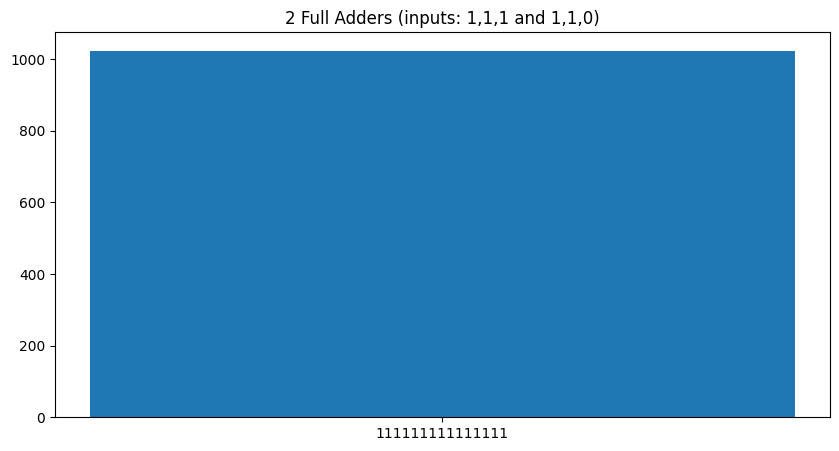
\includegraphics[width=1.00\textwidth]{imagens/simulation-without-noise.png}
        
        imagem 9: resultados da simula\c{c}\~ao sem ru\'ido
        
        \end{figure}

        Como esperado todos os qbit's medidos tem valor 1.

        \begin{figure}[H]
        
        \centering
        
        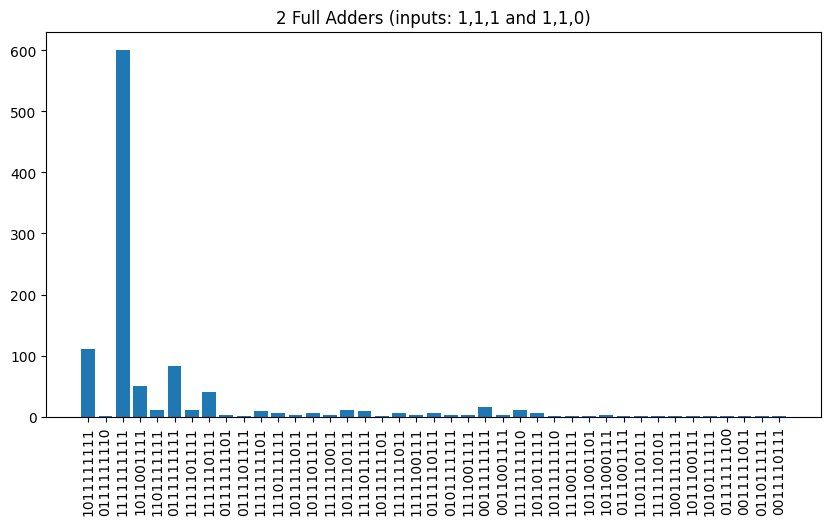
\includegraphics[width=1.00\textwidth]{imagens/simulation-with-noise.png}
        
        imagem 10: resultados da simula\c{c}\~ao com ru\'ido
        
        \end{figure}

        O ru\'ido simulado gerou alguns resultados diferentes - contudo o resultado majorit\'ario ainda \'e o correto.
        
        \begin{figure}[H]
        
        \centering
        
        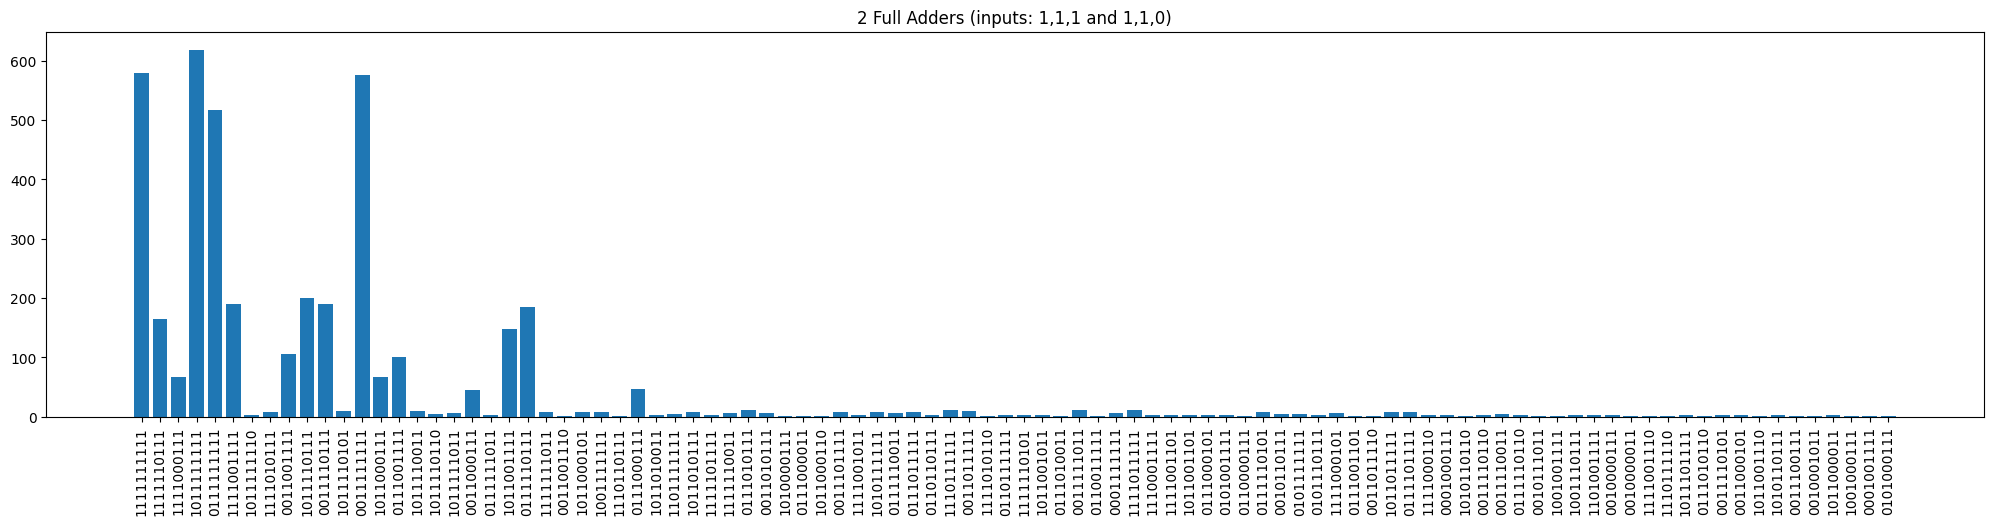
\includegraphics[width=1.00\textwidth]{imagens/real-run.png}
        
        imagem 11: resultados da rotina no computador qu\^antico da IBM (filtrando apenas os resultados com frequ\^encia superior a 10)
        
        \end{figure}

        Note que apesar de haverem v\'arios resultadados com alta frequ\^encia - o resultado de maior frequ\^encia é o resultado correto.
    
    \subsection{Conclusão}
    
        O procedimento como um todo foi essencial para o desenvolver uma comprensão completa das propriedade da computa\c{c}\~ao qu\^antica, bem como suas diferen\c{c} para a cumputa\c{c}\~ao cl\'assica. Tais entendimentos ser\~ao fundamentais no entendimento, desenvolvimento de uma rede neural celular qu\^antica.



    
\end{document}